% !TEX root = anticipation_divmrf.tex
\section{Belief Estimation with  rCRF}
\label{theory}
In this section, we develop the Recursive Conditional Random Field (rCRF) to use CRF in a Bayesian filtering setting. rCRF jointly uses rich model of CRF and the recursive nature of the Bayesian filtering to compute an accurate belief. We first define our modelling assumptions in Section~\ref{rcrfdef}, and then we introduce a link between the CRF likelihood and the measurement likelihood in Section~\ref{fromto} in order to compute the posterior belief. In Section~\ref{beliscrf}, we further show that the resulting posterior belief is equivalent to a CRF. Moreover, this equivalence enables efficient computation via the diversity based method \cite{divmbest} developed for CRFs.
\subsection{Recursive Conditional Random Field}
\label{rcrfdef}
%\vspace{\subsectionReduceTop}
Consider a sequential estimation problem in which we are interested in variables $\mathbf{y}^t$ using observations $\mathbf{x}^t$ where $t$ is the temporal variable. In our application, $t$ is the temporal segment id. We note RGB-D camera reading as $\mathbf{x}^t$, and object and activity labels as $\mathbf{y}^t$. We now define the Recursive Conditional Random Field (rCRF) framework for such a problem following the assumptions of Hidden Markov Models.

\begin{mydef}
Let $\mathcal{G}^t=(V^t,E^t)$ be set of graphs indexed by the temporal variable $t$ and $\mathbf{y}^t$ is indexed by the vertices of $\mathcal{G}^t$ as $\mathbf{y}^t=(y^t_v)_{v \in V^t}$. Then, ($\mathbf{x}^{1\ldots T}$,$\mathbf{y}^{1\ldots T}$) is a \textbf{\textit{Recursive Conditional Random Field}} with dynamics $p_v(\cdot|\cdot)$ when

\begin{enumerate}
	\item For each $t$, $(\mathbf{y}^t,\mathbf{x}^t)$ is a CRF over $\mathcal{G}^t=(V^t,E^t)$
%	\item $\mathbf{y^t} \perp \mathbf{y^{t-k}} | {\mathbf{y^{t-1}}} \quad  \forall {k>1}$
\item $p(\mathbf{y}^{t}|\mathbf{y}^{1},\ldots,\mathbf{y}^{t-1}) = p(\mathbf{y}^{t}|\mathbf{y}^{t-1}) \quad  \forall t$ \hfill (Markov)
%\mathbf{y^{t+1}} \perp \mathbf{y^{t-1}} \; | \; {\mathbf{y^{t}}} \quad  \forall t$ \hfill (Markov)
%	\item $\mathbf{y^{t+1}} \perp \mathbf{y^{t-1}} \; | \; {\mathbf{y^{t}}} \quad  \forall t$ \hfill (Markov)
\item $p(\mathbf{x}^t|\mathbf{y}^1,\ldots,\mathbf{y}^t,\mathbf{x}^1,\ldots,\mathbf{x}^{t-1})=p(\mathbf{x}^t|\mathbf{y}^t)\quad  \forall t$ \hfill
%\item $\mathbf{x^t} \perp \mathbf{y^u} | \mathbf{y^t} \quad  \forall {u \neq t}$ \hfill (Measurements are Cond.Ind.)
\item $p(\mathbf{y}^t=\mathbf{y}|\mathbf{y}^{t-1}=\mathbf{y^\prime})=p_v(\mathbf{y}|\mathbf{y^\prime})$ \hfill (stationarity)
\end{enumerate}
%\vspace{-2mm}
$\hfill \blacksquare$
\end{mydef}
\begin{figure}[ht]
%\vspace{-5mm}
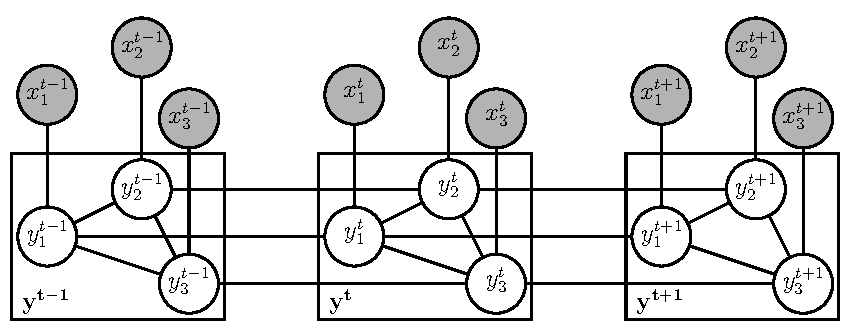
\includegraphics[width=\textwidth]{hmmcrf}
%\vspace{\captionReduceTop}
\caption{{\bf rCRF is defined over a temporal CRF.} The graphical model, we use within the rCRF, is a temporal CRF with additional constraints. We impose a special structure through the conditions we state in the definition. For the visualization purposes, we show there nodes per segment although rCRF can handle any number of nodes.}% Shaded nodes represent the observations.
%\vspace{\captionReduceBot}
\label{rCrf}
\end{figure}

We visualize the graphical model representation of the rCRF in Figure \ref{rCrf}. In this work, we are interested in the belief over state variables at a given time instant $t$ as:
\begin{equation}
bel^t(\mathbf{y}) = p(\mathbf{y}^t=\mathbf{y}|\mathbf{x}_1,\ldots,\mathbf{x}_T) \label{beldef}
\end{equation}
Here, $T$ denotes the length of the video. Hence, in rCRF the belief of any frame is supported by the entire video. Moreover, the time instant $t$ can be greater than the video length $T$ as well. Hence, rCRF naturally supports anticipation setting.
% This problem is typically referred as Bayesian smoothing.

We then decompose the belief by using the independence properties of the rCRF as:
\begin{equation}
bel^t(\mathbf{y}) \propto  \underbrace{p(\mathbf{y}^t=\mathbf{y}|\mathbf{x}^1,\ldots,\mathbf{x}^t)}_{\alpha^t(\mathbf{y})} \underbrace{p(\mathbf{x}^{t+1},\ldots,\mathbf{x}^T|\mathbf{y}^t=\mathbf{y})}_{\beta^t(\mathbf{y})}
\label{beldec}
\end{equation}
Moreover, $\alpha^t$ and $\beta^t$ can be computed recursively by using forward and backward  messages. Following \cite{hmm},
\begin{equation}
\begin{aligned}
\alpha^t(\mathbf{y}^t) &= p(\mathbf{x}^t|\mathbf{y}^t)\sum_{\mathbf{y}^{t-1}} \alpha^{t-1}(\mathbf{y}^{t-1}) p(\mathbf{y}^{t}|\mathbf{y}^{t-1}) \\
\beta^t(\mathbf{y}^t) &= \sum_{\mathbf{y}^{t+1}} p(\mathbf{x}^{t+1}|\mathbf{y}^{t+1}) \beta^{t+1}(\mathbf{y}^{t+1}) p(\mathbf{y}^{t+1}|\mathbf{y}^{t})
\end{aligned}
\label{mespas}
\end{equation}
\noindent
with initializations $\alpha^1(\mathbf{y}^1)=p(\mathbf{x}^1|\mathbf{y}^1)$ and $\beta^T(\mathbf{y}^T)=1$.

\subsection{Computing the belief using an rCRF}
%\vspace{\subsectionReduceTop}
\label{fromto}
Recursive definition in (\ref{mespas}) has two significant drawbacks:
 firstly, CRF is modelling $p(\mathbf{y}^t|\mathbf{x}^t)$ instead of $p(\mathbf{x}^t|\mathbf{y}^t)$ and the transformation is not trivial. Secondly, computation of the messages require a summation over the entire output space, and it has an exponential dimension. In this section, we first compute the posterior of the observation given labels $p(\mathbf{x}^t|\mathbf{y}^t)$ by using the CRF posterior likelihood $p(\mathbf{y}^t|\mathbf{x}^t)$. Then, we show that the belief function at time $t$, $bel^t(\mathbf{y})$, can be approximately represented as a Gibbs measure over $\mathcal{G}^t$. Then, we conclude that the belief, $bel^t(\mathbf{y})$, is a CRF over the graph $\mathcal{G}^t$ with modified energy functions.
%Finally, we suggest a method to efficiently represent the belief over small number of samples in section \ref{divm}.
\subsubsection{From $p(\mathbf{y}^t|\mathbf{x}^t)$ to $p(\mathbf{x}^t|\mathbf{y}^t)$}
Since $(\mathbf{x}^t,\mathbf{y}^t)$ is a CRF, the posterior of the label given the observation follows \cite{geman}; %a Gibbs measure \cite{geman} as;
\begin{equation}
p(\mathbf{y}^t|\mathbf{x}^t) \propto \exp\left( \sum_{i \in V^t} \theta_{x^t_i}(y^t_i) + \sum_{i,j \in E^t} \theta_{x^t_i,x^t_j}(y^t_i,y^t_j)  \right)
\label{crflogl}
\end{equation}
where $\theta$ is the energy function defined over the node set \mbox{$v \in V^t$ }as $\theta_{v}$ and over the edge set \mbox{$(u,v) \in E^t$} as $\theta_{u,v}$.

%\frac{p(\mathbf{y}^t|\mathbf{x}^t)}{p(\mathbf{y}^t)} =
In order to transform  $p(\mathbf{y}^t|\mathbf{x}^t)$ into  $p(\mathbf{x}^t|\mathbf{y}^t)$, we use Bayes rule;
$p(\mathbf{x}^t|\mathbf{y}^t) \propto  \frac{p(\mathbf{y}^t|\mathbf{x}^t)}{ \sum_{x^t} p(\mathbf{y}^t|\mathbf{x}^t)p(\mathbf{x}^t)}$ and compute $p(\mathbf{y}^t)$ as; %the denominator as;
\begin{equation}
p(\mathbf{y}^t)=\sum_{\mathbf{x}^t} \exp\left( \sum_{i \in V^t} \theta_{x^t_i}(y^t_i) + \sum_{i,j \in E^t} \theta_{x^t_i,x^t_j}(y^t_i,y^t_j) \right) p(\mathbf{x}^t)
\end{equation}
For tractability, we approximate the $p(\mathbf{y}^t)$ with its lower bound after applying the Jensen inequality as;
\begin{equation}
	\small
p(\mathbf{y}^t) \approx \exp ( \sum_{i \in V^t} \underbrace{\sum_{\mathbf{x}^t} \theta_{x^t_i}(y^t_i)  p(\mathbf{x}^t)}_{\tilde{\theta}(y^t_i)} + \sum_{i,j \in E^t} \underbrace{ \sum_{\mathbf{x}^t}  \theta_{x^t_i,x^t_j}(y^t_i,y^t_j) p(\mathbf{x}^t)}_{\tilde{\theta}(y^t_i,y^t_j)} )
\end{equation}

% \todo{
We then estimate the inner summations $\tilde{\theta}(\cdot)$
% , expectation over $\mathbf{x}$, )
% empirically by
from the training data
% In other words, we
using Monte Carlo method
% to compute inner summations
 as \mbox{$\tilde{\theta}(\cdot) = \frac{1}{N}\sum_{i=1}^N \theta_{\mathbf{x}^{(i)}}(\cdot)$} where $N$ is the number of training samples and $\mathbf{x}^{(i)}$ is the $i^{th}$ training sample.
 %  with abuse of notation.
 Therefore, we can compute the observation likelihood as:  $p(\mathbf{x}^t|\mathbf{y}^t) \propto$
\begin{equation}\small
\exp\left( \sum_{i \in V^t} \theta_{x^t_i}(y^t_i) - \tilde{\theta}(y^t_i) + \sum_{i,j \in E^t} \theta_{x^t_i,x^t_j}(y^t_i,y^t_j) - \tilde{\theta}(y^t_i,y^t_j)  \right)
\label{obsprob}
\end{equation}

\subsubsection{Belief is a CRF}
\label{beliscrf}
Here we compute the belief (\ref{beldec}) in terms of forward and backward messages and CRF likelihood. We then show that the posterior belief is a CRF. This observation enables us to use efficient methods developed for CRFs.

In order to compute the belief (\ref{beldec}), we decompose
% assume that
% start with the simplifying assumption that
the system dynamics using the independence assumption in the graph in Fig.~\ref{rCrf}.
This gives us \mbox{$p(\mathbf{y}^t|\mathbf{y}^{t-1})=\prod_{i} p(y^t_i|y^{t-1}_i)$}.
% In other words, the system dynamics model does not model correlations
%
% we model the relationship between variables via CRF and do not consider them while modelling temporal dynamics.
%
%After decomposing the state transition dynamics,
We then compute the belief function as \mbox{$bel(\mathbf{y}^t)=\alpha^t(\mathbf{y}^t)\beta^t(\mathbf{y}^t)$} by using equations (\ref{mespas}) and (\ref{obsprob}). After algebraic manipulations, the belief function can be approximated as follows (see supplementary material for a detailed derivation):
\iffalse
\begin{equation}\small
	\begin{aligned}
&bel(\mathbf{y}^t) \propto \exp\left[  \sum_{i,j \in E^t} \left( \theta_{x^t_i,x^t_j}(y^t_i,y^t_j) - \tilde{\theta}(y^t_i,y^t_j) \right) \right. \\
&\left. \sum_{i \in V^t} \left( \theta_{x^t_i}(y^t_i) - \tilde{\theta}(y^t_i) +  \sum_{\mathbf{y^{t-1}}} \alpha^{t-1}(\mathbf{y}^{t-1}) \log p(y^t_i|y^{t-1}_i) \right. \right. \\
&+\left.\left.\sum_{\mathbf{y}^{t+1}} \beta^{t+1}(\mathbf{y}^{t+1}) p(\mathbf{x}^{t+1}|\mathbf{y}^{t+1}) \log p(y^t_i|y^{t-1}_i) \right) \right]
\end{aligned}
\label{crfbelief}
\end{equation}
\fi

\begin{equation}\small
  \begin{aligned}
&bel(\mathbf{y}^t) \propto \exp\left[  \sum_{i,j \in E^t} \left( \theta_{x^t_i,x^t_j}(y^t_i,y^t_j) - \tilde{\theta}(y^t_i,y^t_j) \right) \right. \\
&\left. \sum_{i \in V^t} \left( \theta_{x^t_i}(y^t_i) - \tilde{\theta}(y^t_i) +  \sum_{\mathbf{y}^{t-1}} \alpha^{t-1}(\mathbf{y}^{t-1}) \log p(y^t_i|y^{t-1}_i) \right. \right. \\
&+\left.\left.\frac{1}{\gamma}\sum_{\mathbf{y}^{t+1}} \beta^{t+1}(\mathbf{y}^{t+1}) p(\mathbf{x}^{t+1}|\mathbf{y}^{t+1}) \log p(y^{t+1}_i|y^{t}_i) \right) \right]
\end{aligned}
\label{crfbelief}
\end{equation}
where $\gamma=\sum_{\mathbf{y}^{t+1}} \beta^{t+1}(\mathbf{y}^{t+1}) p(\mathbf{x}^{t+1}|\mathbf{y}^{t+1})$

One property to observe is the decomposition of the belief over the graph. Resulting belief function, (\ref{crfbelief}), is a summation over energy terms defined over nodes $i \in V^t$ and edges $i,j\in E^t$. Hence, belief $bel^t(\cdot)$ is a Gibbs measure over $\mathcal{G}^t$. By using Hammersley-Clifford theorem \cite{hc1971}, we  conclude that the posterior belief in rCRF is also a CRF. In other words, belief is a CRF defined over the same graph with a modified energy.

%\vspace{\sectionReduceBot}
\subsubsection{Belief via Diverse-Most-Likely Samples}
%\vspace{\sectionReduceTop}
\label{divm}
Since we computed the belief function and showed that it is equivalent to a CRF, we now need
an efficient method for computing it.

% here we use an existing method, computing diverse-most-likely samples \cite{divmbest}, that is developed for a CRF, in order to efficiently compute the belief.

We follow the observation that CRF-likelihood over a natural scene concentrates on a few diverse samples \cite{divmbest} because each scene only has a few plausible explanation. So, we compute the belief for only those samples. In other words, let's assume the set of all plausible solutions at time $t$ is $\mathbf{Y}^t={\mathbf{y}^{t,1},\ldots,\mathbf{y}^{t,M}}$ where $\mathbf{y}^{t,i}$ is the $i^{th}$ sample at time $t$. We then redefine the belief as;

\begin{equation}
	\text{approx\_bel}^t(\mathbf{y})=\left\{ \begin{array}{cc} \frac{bel^t(\mathbf{y})}{\sum_{\mathbf{y}^\prime \in \mathbf{Y}^t} bel^t(\mathbf{y}^\prime)} & \text{if $\mathbf{y} \in \mathbf{Y}^t$} \\ 0 & \text{o.w.} \end{array} \right.
\end{equation}

Since there are only a few plausible explanation of a visual observation and CRF-based belief concentrates only on those samples, proper selection of the samples $\mathbf{Y}^t$ is expected to work well in practice. These samples are typically selected as the diverse-most-likely solutions of the CRF. They are most-likely samples because we are only interested in the plausible explanations. They are diverse because we are interested in the modes of the CRF other than set of samples around the MAP solution. Diversity is achieved via asserting samples to be at least $\delta$ unit apart from each other via the distance function $\Delta$ (we use hamming distance as a in our experiments). In other words, we solve the following optimization problem in order to get the samples which represent the belief;
\begin{equation}
\begin{aligned}
\mathbf{y}^{t,i} &= \argmax_{\mathbf{y}}  bel^t(\mathbf{y}) \\
&s.t.\,\, \Delta(\mathbf{y},\mathbf{y}^{t,j}) \geq \delta \quad \forall \; {j < i}
\end{aligned}
\label{divopt}
\end{equation}
%where $\bf{y}^{t,i}$ is the $i^{th}$ sample in the $t^{th}$ frame.
This optimization is NP-hard in general; however, since we already showed $bel^t(\bf{y})$ is CRF, we use the existing diverse-m-best algorithms developed for CRFs. We use the Lagrange relaxation by Batra et al. \cite{divmbest}. We explain the details of solving this problem by using \cite{divmbest} in supplementary material.

In summary, we first compute the belief via (\ref{crfbelief}) for all frames by using samples of the previous and the next frame as well as CRF likelihoods. Then, we compute the diverse samples of (\ref{crfbelief}) by using \cite{divmbest}. After computing the samples, we compute the messages $\alpha^t$ and $\beta^t$ by using the equations (\ref{obsprob}) and (\ref{mespas}). We continue to re-sample the beliefs and re-compute the messages recursively until the convergence. Moreover, during the initialization, we only sample the observation function (\ref{obsprob}) since the messages are not available.
%\vspace{\subsectionReduceBot}
